\section{Příprava vzorku dat pro další analýzy}
\label{sec:priprava}
Data z~výše popsaných tabulek bylo potřeba sloučit do jedné tabulky, aby nad nimi bylo možné provést analýzy. Napojení dat bylo provedeno v~Jupyter Noteboocích v~jazyce Python. Na tabulku s~evidovanými shrinky bylo třeba napojit číselníky. Podle názvů prodejen byly napojeny na prodejny demografické údaje. Údaje o počtu obyvatelích, jsem rozdělila do pěti kategorií. Z~data transakce bylo extrahováno datum pro den a na základě jeho hodnoty bylo určeno do jaké čtvrtiny měsíce patří. Z~data také bylo odvozeno o jaký den v~týdnu se jedná pomocí funkce v~Python knihovně \emph{pandas}.

Na data se zaznamenanými shrinky jsem napojila data o promoakcích a každý řádek označila jednou ze tří hodnot -- žádná promoakce, promoakce, po promoakci. Hodnota \emph{po promoakci} označuje záznamy, které byly evidovány do jednoho týdne po ukončené promoakci na dané prodejně pro daný produkt. 


Zkoumaný dataset se záznamy shrinků produktů jsem rozšířila o další sledované sloupce, které dávají do srovnání hodnotu shrinku a objem tržeb. Vytvořila jsem takto sloupce: 
\begin{itemize}
    \itemsep 0em
    \item Podíl shrinku na celkových tržbách prodejny
    \item Podíl shrinku na tržbách shrinkovaného produktu na prodejně
    \item Podíl shrinku a tržeb v~kategorii úrovně 1 na prodejně
\end{itemize}

Hodnoty ve sloupci byly vypočítány jako hodnota shrinku na jednom řádku vydělená příslušnými tržbami. 
    Tabulka tržeb byla získaná z~tabulky \emph{transakce}, pro ID transakcí, které odpovídají prodejům. Tabulka byla agregovaná podle sloupců: prodejna, čtvrt měsíce, kategorie první úrovně.

S tržbami produktu souvisí i sloupec Prodej, který nabývá logických hodnot \emph{true, false}, podle toho, zda se produkt v~dané období vůbec prodával nebo ne.
% Následující část text bude věnována rozboru dat pro typ shrinku \emph{prošlé a zkažené zboží} pro kategorie Velmi čerstvé a Čerstvé z~produktové hierarchie úrovně 1.
% v~období jednoho kalendářního měsíce.

% \subsection{Rozbor dat}

% Vzhledem k~rozsáhlosti dat bylo třeba zjistit, které proměnné mohou ovlivňovat hodnotu shrinku a které proměnné jsou redundantní. 
% Vzhledem k~vysokému počtu dat pro jeden kalendářní rok, 
% v~roce 2022 bylo v~databázi evidováno přes 32 milionů záznamů o týkající se shrinků
% , jsem se rozhodla provést analýzu na měsíčním výběru dat z~tohoto období. Jako zkoumaný měsíc jsem vybrala měsíc říjen, neboť v~porovnání s~letními měsíci a Vánocemi se v~říjnu nevyskytují významné sezónní výkyvy.

Zkoumaná březnová data obsahují přes $1{,6}$ milionů řádků.
Každý řádek odpovídá jednomu záznamu v~databázi shrinku daného produktu. Sledované údaje ve sloupcích\footnote{Překlady sloupců do angličtiny jsou uvedeny v příloze práce.} jsou: 
% \subsubsection{Sledované údaje}
\begin{itemize}
    \itemsep-0.34em
    \item ID prodejny -- kategorická proměnná
    \item Typ prodejny -- kategorická proměnná
    \item Okres -- kategorická proměnná
    \item Kraj -- kategorická proměnná
    \item Počet obyvatel v~lokalitě -- kategorická proměnná
    \item ID produktu -- kategorická proměnná
    \item Datum transakce -- kategorická proměnná
    \item ID shrinku -- kategorická proměnná
    \item 1 (úroveň) -- kategorická proměnná
    \item 2 (úroveň) -- kategorická proměnná
    \item 3 (úroveň) -- kategorická proměnná
    \item 4 (úroveň) -- kategorická proměnná
    \item 5 (úroveň) -- kategorická proměnná
    \item 6 (úroveň) -- kategorická proměnná
    \item Typ promoakce -- kategorická proměnná
    \item Prodej\footnote{Příznak \emph{prodej} je v~implementaci označen jako \emph{sales}.} -- kategorická proměnná
    % \item Expirace -- kategorická proměnná
    \item Den v~týdnu -- kategorická proměnná
    % \item Číslo dne -- kategorická proměnná
    \item Čtvrt měsíce (rozdělení měsíce na čtyři části) -- kategorická proměnná
    \item Množství -- spojitá proměnná
    \item Ztracené náklady (označováno také jako hodnota shrinku) -- spojitá proměnná
    \item Podíl na tržbách produktu -- spojitá proměnná
    \item Podíl na celkových tržbách -- spojitá proměnná
    \item Podíl na tržbách kategorie z~úrovně 1 -- spojitá proměnná
\end{itemize}
% Původní sloupec datum jsem rozdělila ještě na dvě jiné proměnné, a to den v~týdnu a období v~měsíci.
%  a sloupec datum jsem vynechala. 


\subsection{Výběr dat}
% výběr dle zastoupení shrinků a kategorií produktů a dle outlierů.

Nejprve jsem graficky analyzovala zastoupení shrinků v~závislosti na vybraných proměnných pomocí nástroje Power BI, viz obr. \ref*{obr:rok:g:zastoupeni1} a \ref*{obr:rok:g:zastoupenish1}. Více o analýze v~tomto nástroji je v~kapitole \ref{ch:vizualizace}. V~návaznosti na zjištěné zastoupení shrinků v~datech jsem se rozhodla vybrat pouze nejvíce zastoupený typ shrinku, který tvoří více jak 62~\% celkových nákladů. Ponechaný byl tedy pouze shirnk \emph{prošlé a zkažené zboží}. Sloupec s~ ID shrinku lze proto z~dat vynechat.

\begin{figure}[h!]
    \centering
    \captionsetup{justification=centering}
    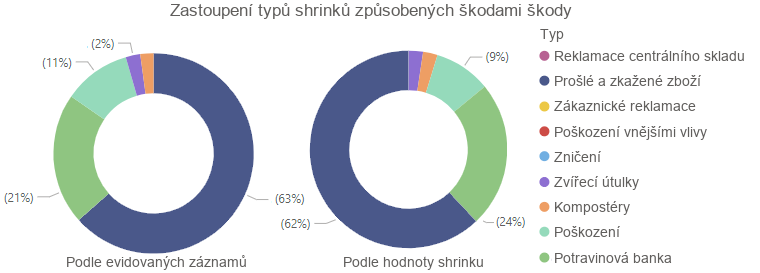
\includegraphics[width=0.96\textwidth]{obrazky/grafy/zastoupenishrinky.png}
    \caption{Zastoupení typů shrinků způsobených škodami v~datech \\ z~března roku 2023 podle hodnoty shrinku.}
    \label{obr:rok:g:zastoupenish1}
\end{figure}

Obdobně jsem přistupovala k~záznamům i z~hlediska kategorie produktu úrovně 1, jelikož z~grafu je patrné, že majoritní zastoupení mají pouze dvě kategorie, a to kategorie Velmi čerstvé a Čerstvé. Všechny záznamy se zbylými kategoriemi jsem z~datasetu pro další analýzy odstranila. Těmito kroky byl zredukován původní počet řádků datasetu na % TODO ověřit číslo
necelých jeden a půl milionu řádků.

\begin{figure}[h!]
    \centering
    \captionsetup{justification=centering}
    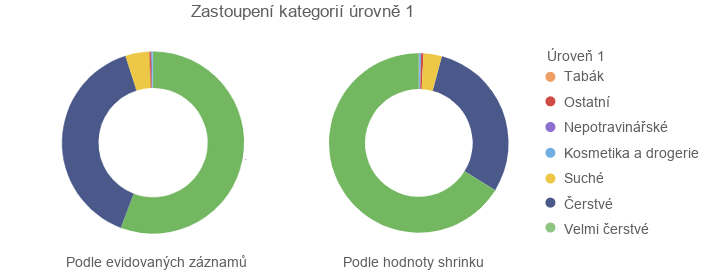
\includegraphics[width=0.98\textwidth]{obrazky/grafy/zastoupeniL1.png}
    \caption{Zastoupení kategorií úrovně 1 v~datech \\ z~března roku 2023 podle hodnoty shrinku.}
    \label{obr:rok:g:zastoupeni1}
\end{figure}

Jako cílové sloupce (\emph{target}) jsem určila sloupce s~ množstvím produktu, hodnotou shrinku a podíly. Zbylé sloupce slouží jako vysvětlující proměnné, dále budou označovány jako příznaky pro cílové sloupce. Všechny vybrané příznaky jsou kategorické proměnné, které lze dále rozdělit na nominální a ordinální. Nominální proměnné jsou ID prodejny, typ prodejny, typ promoakce, prodej, ID produktu, kategorie produktové hierarchie a údaje o lokalitách. Ordinální proměnné jsou den v~týdnu a období měsíce. Ordinální příznaky jsem přeznačila tak, aby každá obsahovala pouze hodnoty od nuly do $n_p$, kde $n_p$ je počet kategorií v~$p$-tém příznaku. 

Pro další postup bylo vhodné přesunout se z~nominálních kategorických hodnot na číselné hodnoty. Pro tyto účely jsem zvolila metodu kódování podle cílového sloupce.  %!!! TODO odkaz do teorie, princip meotdy je vysvětlený v~kapitole...
Neboť toto kódování na numerické hodnoty zachovává velikost datového souboru, to je klíčové vzhledem k~tomu, že nominální proměnné ve zkoumaných datech obsahují velký počet kategorií. 
Např. počet unikátních produktů v~datech je více než 19 tisíc, což odpovídá stejnému počtu kategorií pro tuto proměnnou. Pokud bych použila one-hot kódování\footnote{One-hot kódování převádí kategorické hodnoty na numerické tak, že pro každou kategorii vytvoří samostatný sloupec s~binárními hodnotami, kde 1 odpovídá dané kategorii a 0 zbylým kategoriím.}  mohlo by dojít k~zásadnímu zvýšení počtu sloupců v~datech, v~tomto případě až o desítky tisíc. Kódování podle cílového sloupce je podobné převodu, který jsem použila pro ordinální proměnné. Avšak na rozdíl od něj, hodnota, která je kategorii přiřazena, souvisí se zastoupením této skupiny v~cílovém sloupci a nesouvisí s~uspořádáním hodnot uvnitř příznaku. Nevýhodou je, že takto upravená data mohou být náchylná na overfitting a zanést do vysvětlujících proměnných nové informace o vysvětlované proměnné. 
% proto je potřeba při predikování použít křížovou validaci.\cite{bib:encoding}

% warehouse_id 339
% product_id 19026
% date_of_transaction 31
% motive_type 10
% cost_value 173409
% 1 7
% 2 20
% 4 141
% 5 450
% 6 1369
% expirace 330
% amount 48634
% weekday 7
% day 31
% quarter_of_month 5

Dále jsem se zabývala identifikací odlehlých hodnot. Nejprve jsem vizualizovala hodnoty pomocí grafu. Ukázka grafu je na obr. \ref*{obr:rok:g:outlierN}. Z~grafu je patrné, že problémová je proměnná s~ID prodejny. Prodejny, které tvoří outliery mohou být malé prodejny, které kvůli menšímu počtu celkových produktů neevidují větší počet shrinků. % !!! TODO jakeho grafu 

\begin{figure}[hbtp!]
    % \centering
    % \begin{minipage}{.5\textwidth}
        \centering
        \captionsetup{justification=centering}
        
        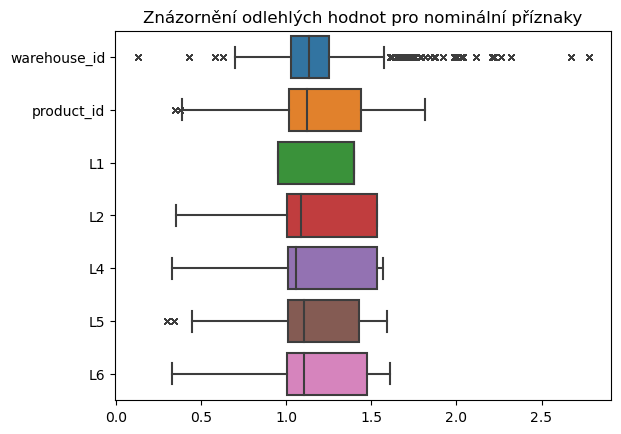
\includegraphics[width=.6\textwidth]{obrazky/zntb/box_nominal.png}
        \caption{Znázornění odlehlých hodnot pro vybrané nominální příznaky.}
        \label{obr:rok:g:outlierN}
    % \end{minipage}%
    % \begin{minipage}{.5\textwidth}
    %     \centering
    %     \captionsetup{justification=centering}

    %     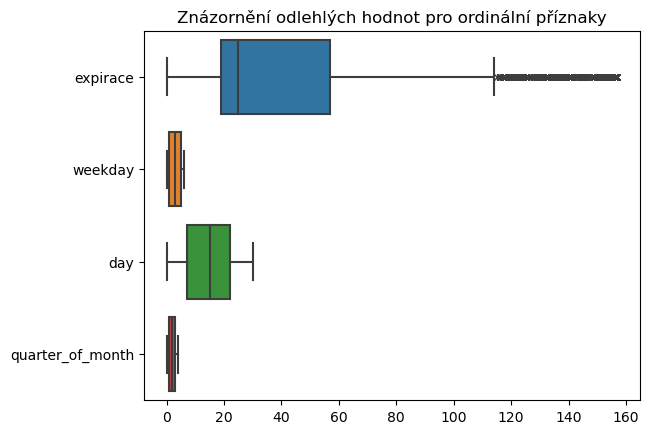
\includegraphics[width=.98\textwidth]{obrazky/zntb/box_ordinal.png}
    %     \caption{Znázornění odlehlých hodnot pro nominální příznaky.}
    %     \label{obr:rok:g:outlierO}
    % \end{minipage}
\end{figure}

Pomocí Tukeyho testu, implementovaného v~jazyce Python, jsem identifikovala přes $150\ 000$ outlierů pro příznak ID prodejny %(\texttt{warehouse\_id})
, čímž se dataset zredukoval. S~tímto krokem klesl i počet ostatních outlierů.

V dalším kroku jsem se zaměřila na míru závislosti mezi proměnnými. Použitým metodám je věnována sekce v~teoretické části \ref{sec:Teoriekorelace}. 
Pro měření závislosti jsem již pracovala s~kategorickými hodnotami proměnných, tj. bez převodu na spojité hodnoty. Důvodem je to, že když jsem provedla měření korelace na překódovaných datech, byla míra zavislosti ovlivněna cílovým sloupcem, který byl použitý pro kódování.
% Vizualizovala jsem data pomocí scatter matice pro všechny proměnné, matice je možné vidět na obr. č. \ref*{obr:nb:scatter}. Z~této matice můžeme na první pohled vidět, že příznaky odpovídající produktové hierarchii a ID produktu vykazují závislost, což plyne z~definice uspořádání této hierarchické kategorizace. V~následujících krocích je cílem vybrat tu kategorii, která nejlépe popisuje data ve vztahu k~shrinkům.

% \begin{figure}[h!]
%     \centering
%     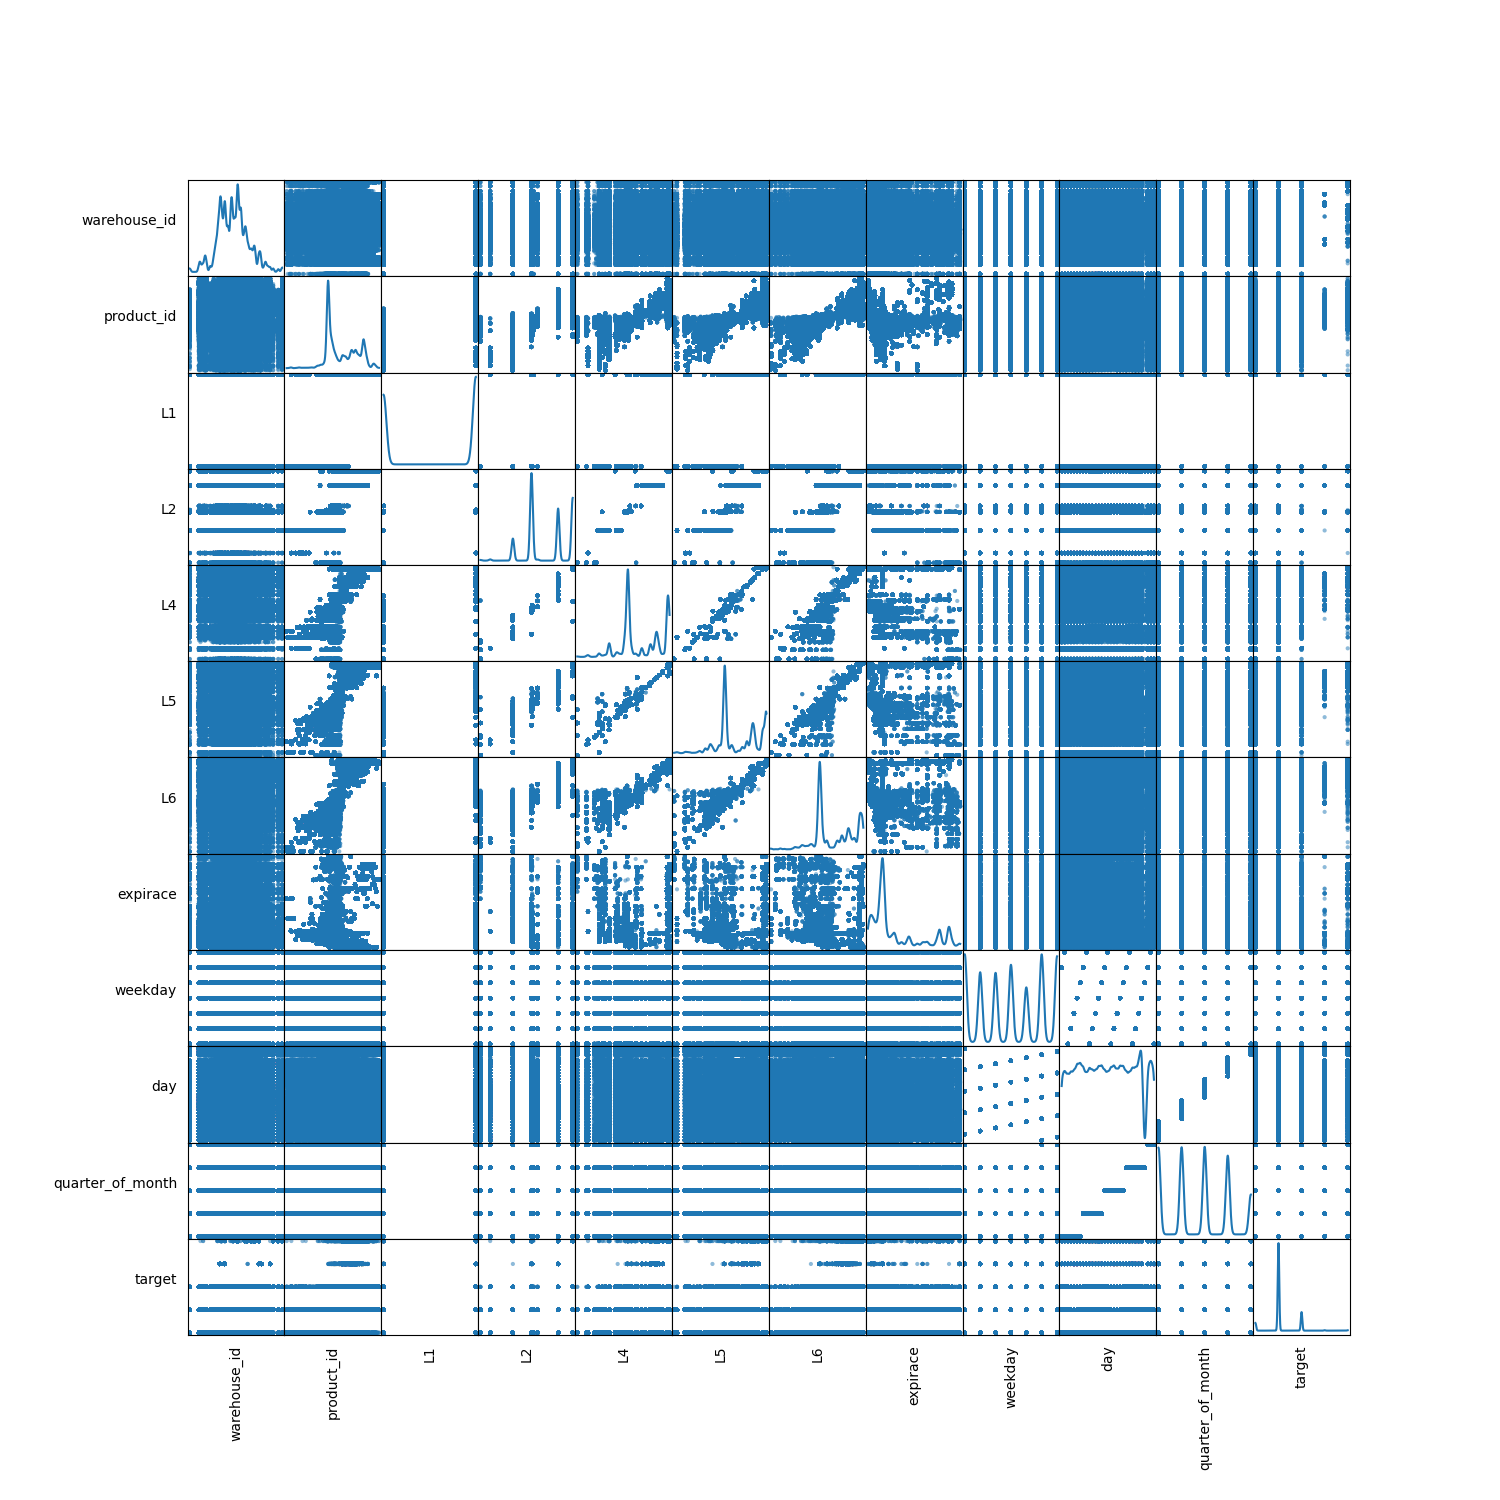
\includegraphics[width=.8\textwidth]{obrazky/zntb/MyScatter.png}
%     \caption{Scatter matice příznaků.}
%     \label{obr:nb:scatter}
% \end{figure}
 
Jako první metodu jsem zvolila  $\chi^2$ statistiku. Vzhledem k~vysokému počtu dat je matice příliš řídká, a proto nejsou výsledné hodnoty vypovídající a test je tedy pro tuto úlohu nespolehlivý.
% Jiným měřítkem pro korelaci mezi proměnnými je Pearsonův korelační koeficient. % odkaz na teorii
% Výslednou matici popisující korelační vztahy mezi příznaky jsem vizualizovala teplotní mapou, která je zobrazena na obrázku \ref*{obr:nb:pearson}. Z~výsledků je opět patrné, že mezi jednotlivými kategoriemi produktů a produkty je silná korelace. Toto zjištění je logické, neboť se jedná o stromovou strukturu kategorií. Zároveň existuje korelace mezi produktovými kategoriemi a expirací produktu. $p$-hodnota odpovídající jednotlivým koeficientům byla vždy nulová, kromě pro koeficient týkající se dvojice proměnných expirace a ID prodejny a expirace a pořadí dne v~týdnu. Je tedy možné považovat výsledky (kromě těchto dvou výjimek) za statisticky významné.

% \begin{figure}[hbtp!]
%     \centering
%     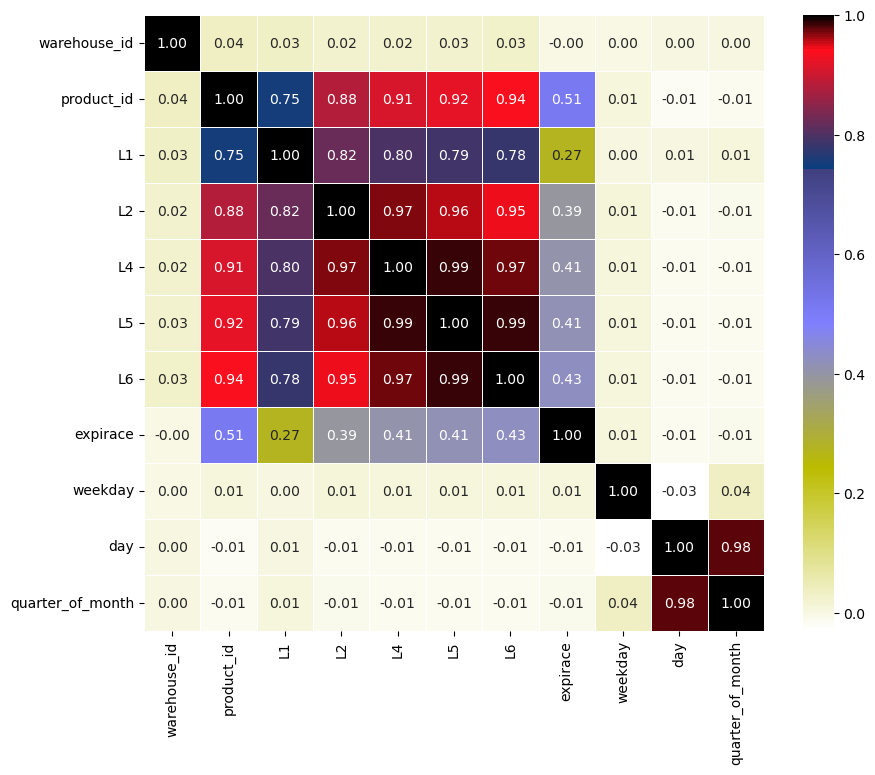
\includegraphics[width=.8\textwidth]{obrazky/zntb/pearson.png}
%     \caption{Matice korelačních koeficientů mezi příznaky.}
%     \label{obr:nb:pearson}
% \end{figure}
Použila jsem proto míru vzájemné informace, která říká, jaká je podobnost mezi dvěma proměnnými \cite{bib:scikit}.
Matice vypočítaných koeficientů je na obr. \ref*{obr:nb:MI}. Jedná se o symetrickou vlastnost, proto jsou hodnoty pod a nad diagonálou stejné. Z~výsledků je opět vidět, že ID produktu sdílí informaci s~úrovněmi kategorizace tím více, čím je kategorizace jemnější, což logické z~povahy hierarchického stromu kategorií. Obdobně tomu je i u ID prodejny a údajích o lokalitě a datumových údajích. Jinak jsou hdonoty vzájemné informace nízké.

\begin{figure}[h!]
    \centering
    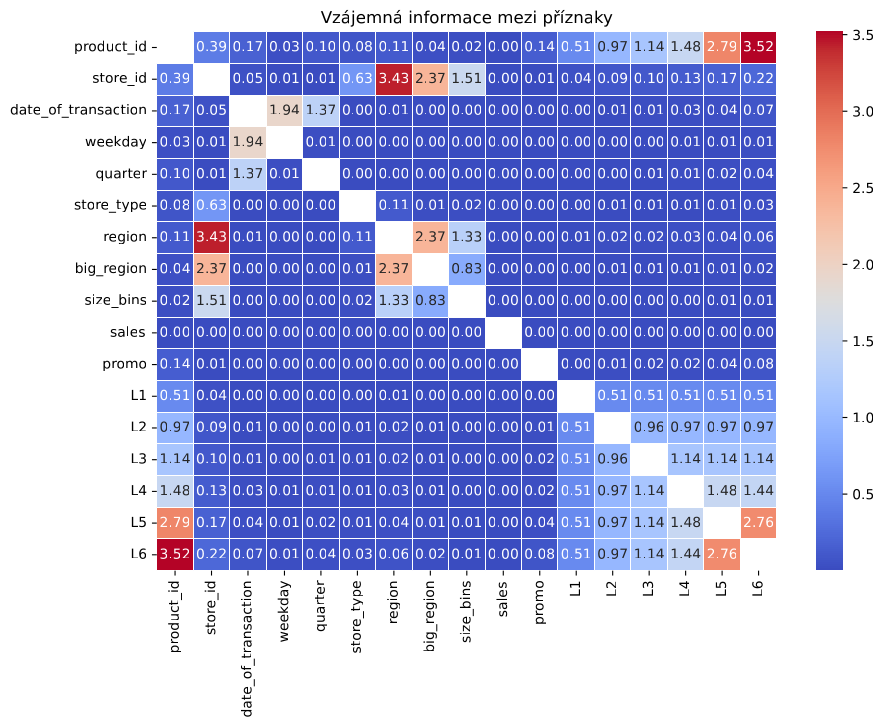
\includegraphics[width=\textwidth]{obrazky/pripravadat/matrix_MI-everything-SFF-storesFETURES-002.png}
    \caption{Matice koeficientů vzájemné informace mezi příznaky.}
    \label{obr:nb:MI}
\end{figure}

Dále jsem pro znázornění vztahu mezi proměnnými použila koeficient Cramerovo $V$. Koeficient jsem postupně počítala pro každou dvojici příznaků. Koeficient nabývá hodnot mezi 0 a 1. Číslo blízké nule indikuje, že mezi proměnnými není asociace, číslo blízké jedničce vysokou závislost \cite{bib:statology}. Na obr. \ref*{obr:nb:cramers} lze vidět, že pro kategorie 1 až 6 a ID produktu je hodnota koeficientu po zaokrouhlení vždy rovna jedné. Vysoká závislost je pak i mezi příznakem promoakce a ID produktu. Dále logicky mezi datem transakce a dnem v~týdnu a obdobím v~měsíci. ID prodejny je extrémně závislé s~demografickými údaji o lokalitách a typem prodejny.

Mírná závislost se také ukázala mezi typem promoakce a ID produktu nebo mezi ID produktu a ID prodejny, dále mezi ID prodejny a první úrovní hierarchie.

\begin{figure}[h!]
    \centering
    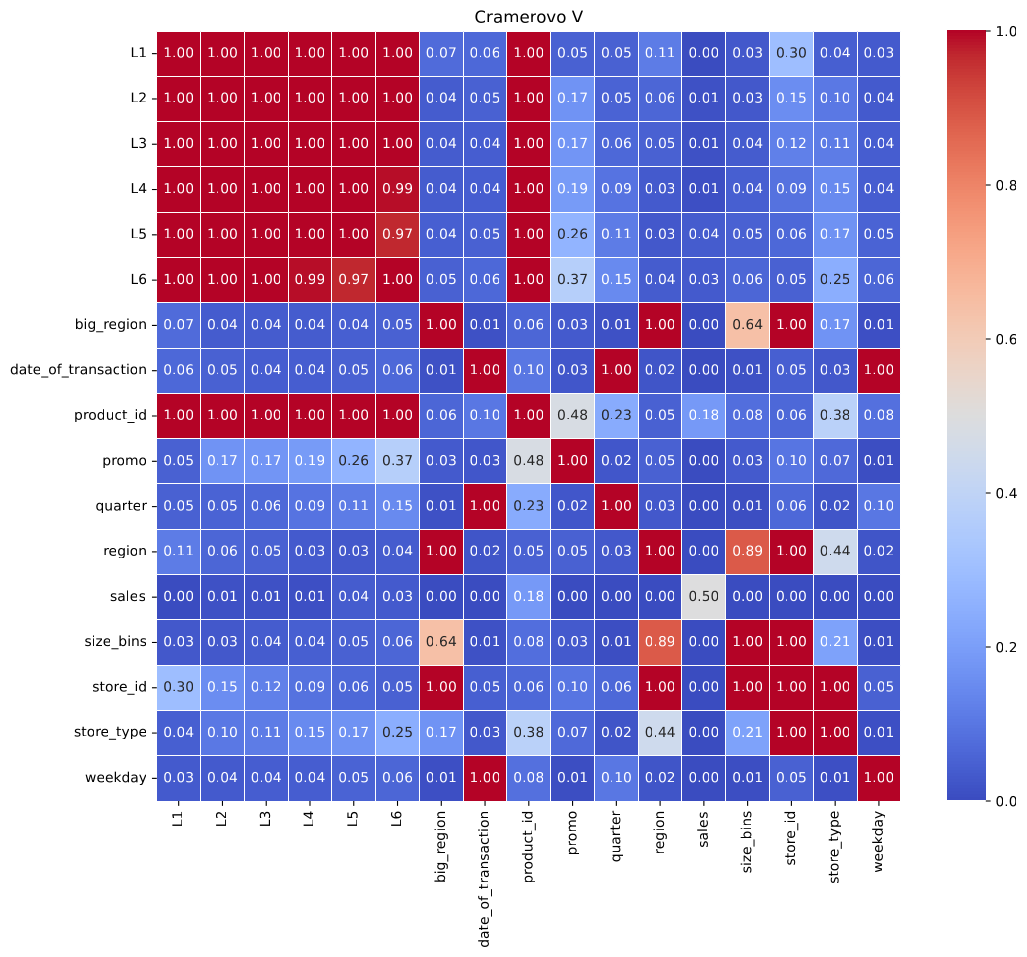
\includegraphics[width=\textwidth]{obrazky/pripravadat/correlation_matrix_cramers-everything-SFF-stores_targets002.png}
    \caption{Matice koeficientů Cramerovo $V$ pro kategorické příznaky.}
    \label{obr:nb:cramers}
\end{figure}

Další statistikou spočtenou na datech je Theilovo $U$ (neboli koeficient nejistoty), který opět nabývá hodnot mezi 0 a 1 a měří vztah mezi dvěma proměnnými. Na rozdíl od předchozích statistik tento koeficient není symetrický a z~výsledků lze vyvodit, ze které proměnné ze dvou zkoumaných můžeme vyvodit informaci o druhé proměnné \cite{bib:correl}. Z~výsledků zobrazených v~matici na obr. \ref*{obr:nb:thiels} plyne, že z~ID produktu lze vyvodit část informace o kategoriích. Zatímco úrovně 1 a 2 o ID produktu mnoho informace nenesou, což logické. Jak bylo ukázáno i v~předchozích statistikách a jak vyplývá z~logiky pro získání dne v~týdnu a období měsíce, číslo dne nese informaci o těchto dvou příznacích.

\begin{figure}[h!]
    \centering
    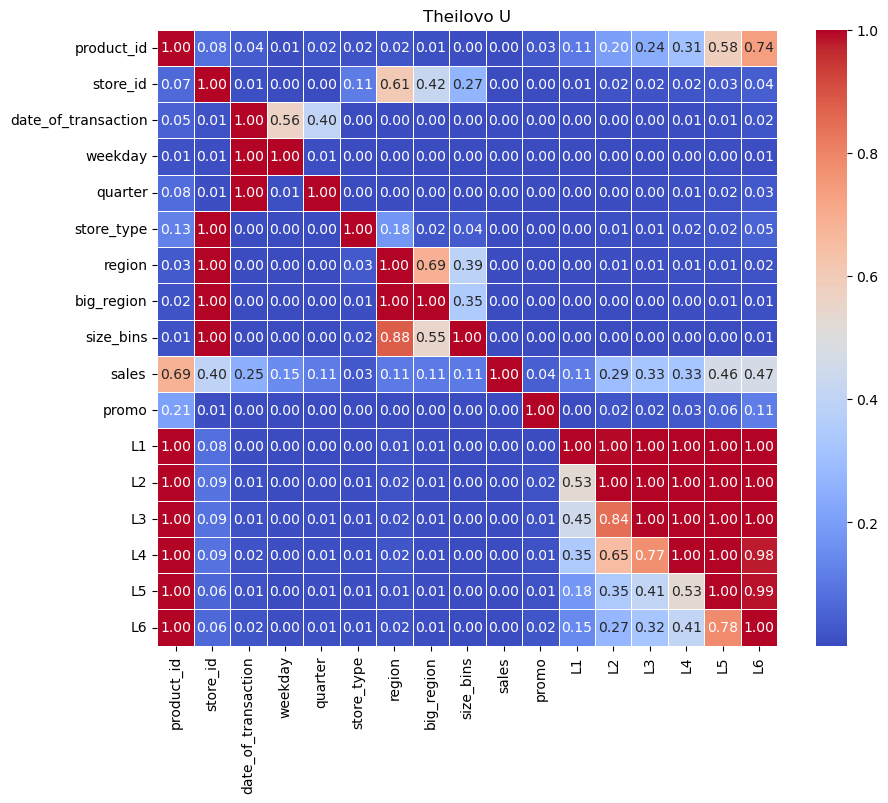
\includegraphics[width=\textwidth]{obrazky/pripravadat/theils_u-002.png}
    \caption{Matice koeficientů Theilovo $U$ mezi příznaky.}
    \label{obr:nb:thiels}
\end{figure}

Z vypočítaných statistik na datasetu je patrné, že některé příznaky jsou významně závislé, a proto je třeba je z~dat odstranit. Kandidáti na vynechání jsou kategorie 2, 3, 5, 6, počet obyvatel a kraj. 
% V~dalších testech budou také vybráni kandidáti a v~závěru vyhodnotím, které příznaky byly podle aplikovaných metod vybrány jako vhodné k~vynechání a které nikoli.
%  TODO  !!!!

V dalším testu jsem otestovala multikolinearitu dat pomocí rozptylového inflačního faktoru (VIF). Jako hraniční faktor jsem zvolila hodnotu 5 VIF, nad kterou již může být závažný problém multikolinearity.\cite{bib:MB}
% TODO opravdu az takhle trochu min
Vysvětlující proměnné jsem odebírala z~datasetu postupně a odebírání jsem ukončila až, když hodnota VIF nebyla nižší než hraniční.
Tímto došlo k~redukci příznaků. Příznaky 1,2,3,5, kraj, prodej, okres měly hodnotu VIF vyšší než 5. Příznaky datum, ID produktu, ID prodejny byly těsně pod hodnotou prahu.
Hodnoty koeficientu VIF na datech jsou na obr. \ref*{obr:nb:vif}. 

\begin{figure}[h!]
      \centering
      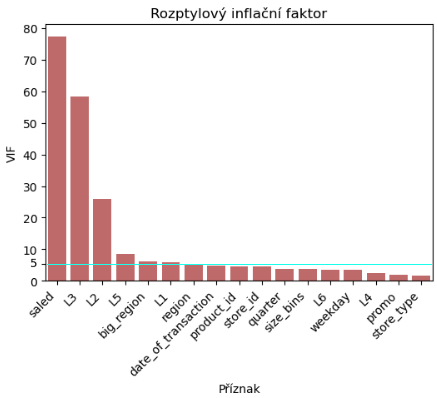
\includegraphics[width=.6\textwidth]{obrazky/zntb/VIF2.png} % SEM DAT NOVY OBRAZEK TODO
      \caption{Rozptylový inflační faktor.}
      \label{obr:nb:vif}

    \end{figure}

Jako další metodu po výběr příznaků jsem vypočítala hodnotu koeficientů vzájemné informace mezi všemi příznaky s~cílovými sloupci. Na obrázku \ref*{obr:nb:MI_FS} lze vidět, jak jednotlivé proměnné souvisí s~cílovými sloupci. 
Zde lze vidět, že příznak ID prodejny nese malou část informace o cílových sloupcích. Nejvíce informace je sdíleno s~ID produktu a kategoriemi. Ostatní příznaky podle tohoto kritéria nemají mnoho společné informace.

\begin{figure}[h!]
    \centering
    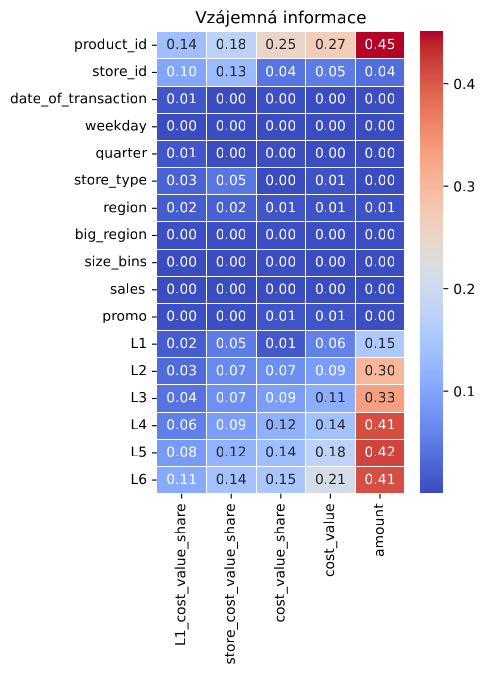
\includegraphics[width=.5\textwidth]{obrazky/pripravadat/matrix_MI-everything-SFF-stores-002.png}
    \caption{Vzájemná informace mezi příznaky cílovými sloupci.}
    \label{obr:nb:MI_FS}

  \end{figure}

Jako hlavní metodu pro výběr proměnných jsem se rozhodla použít metodu PCA, případně MCA. Tuto metodu je možné použít, protože kategorické proměnné byly převedeny na číselné pomocí základního kódování kategorických hodnot na hodnoty 0 až $n$, kde $n$ je počet kategorií v~příznaku. Toto kódování má bohužel tu nevýhodu, že dává kategoriím pořadí, i když jedna kategorie není lepší než jiná. Alternativou je použití metody MCA, která se používá pro kategorické datasety. Výsledky pro metodu MCA jsou uvedeny dále v~textu.
Ve své práci jsem využila implementaci PCA v~knihovně \emph{Prince} v~jazyce Python. 
Předtím než jsem metodu aplikovala jsem otestovala předpoklad homoskedasticity, tedy shodnost rozptylů v~datech, pomocí Bartlettova testu implementovaného v~knihovně \emph{factor\_analyzer}. Nulová hypotéza o shodnosti rozptylů nebyla vyvrácena ($p$-hodnota vyšla nulová). Metodu PCA je proto možné použít.

Na obrázcích \ref*{obr:nb:pca_roztyl_komponetn} a \ref*{obr:nb:pca_kum_roztyl_komponetn} je znázorněno prvních deset komponent a rozptyl který v~datech vysvětlují. 
% Na základě hodnot jsem vybrala prvních deset komponent. 
Desátá komponenta (označená č. 9) spolu s~předchozími vysvětluje téměř 80~\% variability dat. V~dalším kroku jsem vypočítala příspěvky příznaků k~těmto komponentám a vybrala jsem ty příznaky, které přispívají nejvíce. Jejich příspěvek je znázorněný na obr. \ref*{obr:nb:pca_prispevek}. Na základě výsledků analýzy hlavních komponent lze říci, že nejvíce rozptylu v~datech nesou příznaky -- ID prodejny, datum transakce, typ prodejny, počet obyvatel, úroveň L6, čtvrtina mesíce, kraj, ID produktu. Příznaky typ promoakce, den v~týdnu, okres, úroveň 2 a prodej nepřispívají každý ani deseti procenty ke komeponentám.

\begin{figure}[hbtp!]
    \centering
    \begin{minipage}[t]{.466\textwidth}
      \centering
      \captionsetup{justification=centering}

      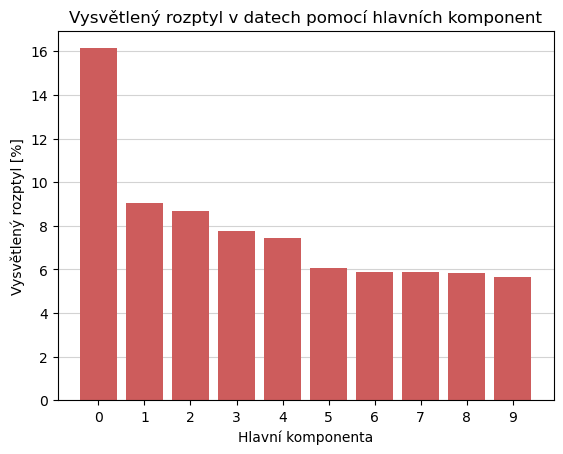
\includegraphics[width=\textwidth]{obrazky/pripravadat/pca-roztyl_komponetn.png}
      \caption{PCA - vysvětlený \\ rozptyl hlavních komponent.}
      \label{obr:nb:pca_roztyl_komponetn}
    \end{minipage}%
    \begin{minipage}[t]{.5\textwidth}
      \centering
      \captionsetup{justification=centering}

      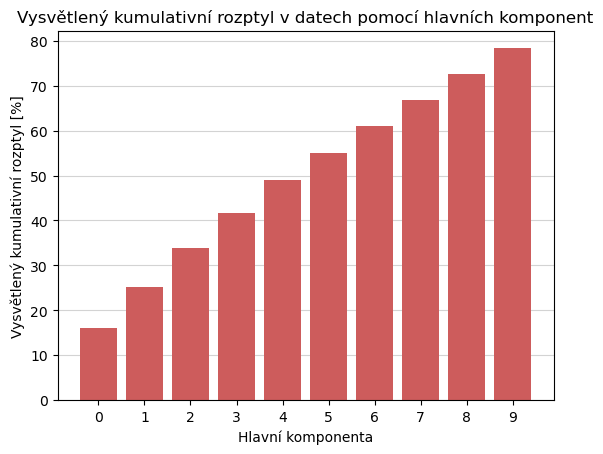
\includegraphics[width=\textwidth]{obrazky/pripravadat/pca-kum_roztyl_komponetn.png}
      \caption{PCA - kumulativní vysvětlený rozptyl hlavních komponent.}
      \label{obr:nb:pca_kum_roztyl_komponetn}
    \end{minipage}
    \end{figure}

\begin{figure}[h!]
    \centering
    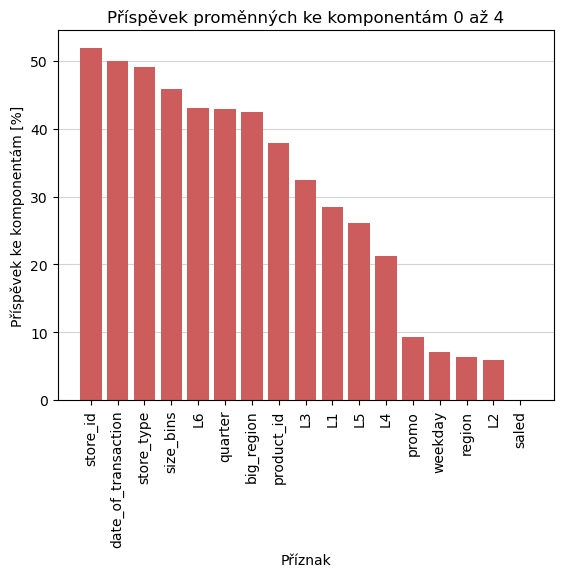
\includegraphics[width=.6\textwidth]{obrazky/pripravadat/pca-prispevky.png}
    \caption{Příspěvek proměnných ke komponentám 0 až 10.}
    \label{obr:nb:pca_prispevek}
\end{figure}
    
Jak již bylo zmíněno pro redukci dimenzionality, příp. výběr proměnných, u kategorických dat lze použít metodu MCA, opět jsem využila implementaci z~knihovny \emph{Prince}. 
V~této implementaci jsou nominální kategorické hodnoty kódovány tak, že narůstá počet sloupců, což náročnější na výpočetní výkon. Vzhledem k~tomu, že jsem analýzy spouštěla na běžném osobním počítači, bylo proto nutné, vzhledem k~nárokům na paměť k~uložení matice, omezit množství dat. Odebrala jsem kategorie 5 a 6, které jsou velmi korelované s~ID produktu a vybrala jsem náhodný 20\% vzorek dat, na které jsem MCA aplikovala. Náhodný výběr jsem několikrát opakovala, aby bylo možné výsledek považovat za důvěryhodný. Ve výsledných příspěvcích ke komponentám se v~závislosti na vybraných datech měnilo pořadí pouze příznaků, které měly blízké hodnoty příspěvku. Příznaky s~malým příspěvkem neměly v~žádném z~provedených běhů vyšší příspěvek než 10 \%. Přesto je třeba brát rozdělení dat v~úvahu při porovnávání výsledků s~jinými metodami.

Vypočítala jsem prvních pět komponent, které dohromady popisují 79~\% variability dat. Jelikož byla každá kategorie chápána jako samostatná proměnná příspěvky jednotlivých příznaků ke komponentám byly rozmístěny mezi všechny kategorie, nikoli k~jednotlivým příznakům, takže je třeba pak příznaky zpětně agregovat.
Po agregaci podle původních příznaků největší příspěvek mělo ID prodejny, okres, ID produktu, kraj a kategorie 4, 3. Zatímco nejmenší datum, den v~týdnu, období měsíce, typ prodejny a prodej. Tyto výsledky je třeba brát se zvážením neboť výpočty probíhaly na řádově menším vzorku než u předchozích metod.
N obrázcích \ref*{obr:nb:mca_roztyl_komponetn} a \ref*{obr:nb:mca_kum_roztyl_komponetn} se nachází výsledky pro jeden běh metody MCA.

\begin{figure}[hbtp!]
    \centering
    \begin{minipage}[t]{.5\textwidth}
      \centering
      \captionsetup{justification=centering}

      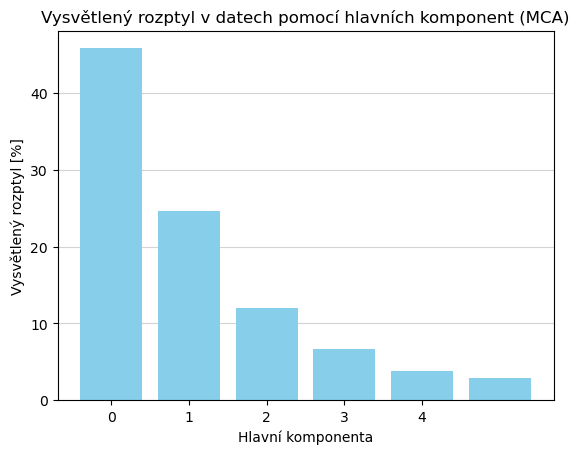
\includegraphics[width=\textwidth]{obrazky/pripravadat/mca-roztyl_komponetn.png}
      \caption{MCA - vysvětlený \\ rozptyl hlavních komponent.}
      \label{obr:nb:mca_roztyl_komponetn}
    \end{minipage}%
    \begin{minipage}[t]{.5\textwidth}
      \centering
      \captionsetup{justification=centering}

      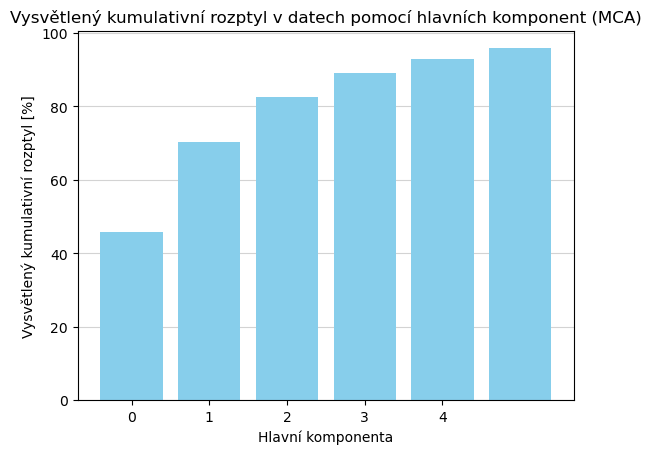
\includegraphics[width=\textwidth]{obrazky/pripravadat/mca-kum_roztyl_komponetn.png}
      \caption{MCA - kumulativní vysvětlený rozptyl hlavních komponent.}
      \label{obr:nb:mca_kum_roztyl_komponetn}
    \end{minipage}
    \end{figure}

\begin{figure}[h!]
    \centering
    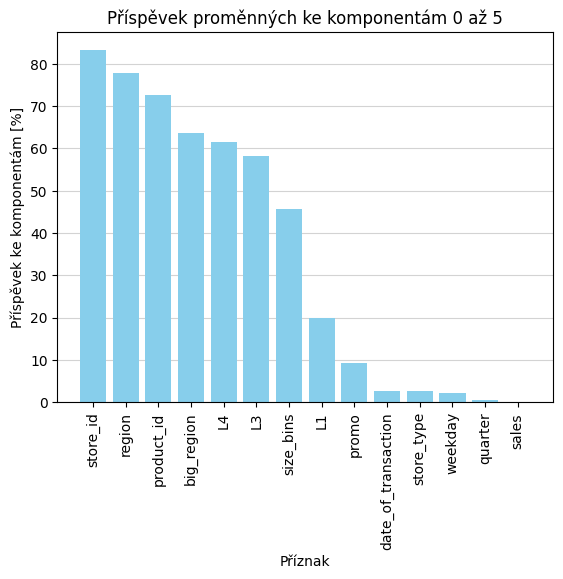
\includegraphics[width=.6\textwidth]{obrazky/pripravadat/mca-prispevky.png}
    \caption{Příspěvek proměnných ke komponentám 0 až 5.}
    \label{obr:nb:mca_prispevek}
\end{figure}


% warehouse_id        0.024256
% product_id          1.147270
% 1                  0.035793
% 2                  0.355452
% 4                  0.841652
% 5                  0.911692
% 6                  0.930902
% expirace            0.306007
% weekday             0.035521
% day                 0.362474
% quarter_of_month    0.048981

\subsection*{Shrnutí pro výběr dat}

Na základě předchozích metod bylo z~původních příznaků datasetu 
vybráno několik příznaků, které popisují hodnotu shrinku.
Vzhledem k~tomu, že různé metody vybraly různé příznaky, níže je sepsáno shrnutí, které říká, jaké příznaku jsou na základě zkoumaných dat relevantní vzhledem k~naměřeným hodnotám shrinku. 

Závislé jsou hodnoty ID produktu a úrovně produktové hierarchie. Dále také z~data lze určit období měsíce i den v~týdnu. ID produktu je závislé s~umístěním prodejny a vlastnostmi lokality a typem prodejny.  Ze zmíněných korelovaných příznaků stačí použít pouze část příznaků, pokud je tato úvaha aplikována na výsledky metod PCA a MCA a výsledků zjištěných pomocí hraniční hodnoty VIF.

Následující sloupce byly získány podle hodnoty rozptylového inflačního faktoru -- úroveň 4, ID produktu, počet obyvatel, období měsíce, typ promoakce, den v~týdnu a prodej. Touto metodou byl navržena i úroveň 6, ta však z~důvodů korelace nebyla zahrnuta. Také hraniční ID prodejny a kraj byly proto vynechány. 
    
Metodou PCA bylo zjištěno, které příznaky nejvíce přispívají ke komponentám, které popisují téměř 96~\% rozptylu v~původních datech. Po vynechání závislých příznaků se jedná o příznaky -- ID prodejny, datum transakce, typ prodejny, počet obyvatel, úroveň L6, čtvrtina měsíce, kraj, ID produktu. 
% Naopak metoda MCA vybrala kategorie 4 až 6 jako důležité. Sloučením a přihlédnutím ke korelačním koeficientům byly vybráno pět příznaků -- 
    % ID prodejny, den v~týdnu, období v~měsíci, 5.


Díky výběru příznaků různými metodami, lze říci, které vlastnosti mohou být důleži-\\té vzhledem k~zjišťování příznaků shrinků ze zaznamenaných dat. Vybrané příznaky mohou sloužit jako základ pro vyslovení hypotéz.

% \begin{enumerate}
%     \item Následující sloupce byly získány podle hodnoty rozptylového inflačního faktoru. Touto metodou byl navržen i sloupec s~číslem dne, ten však z~důvodů korelace nebyl zahrnutý
%     \begin{enumerate}
%         \item[1.1.] 1, období měsíce, ID prodejny a den v~týdnu.
%     \end{enumerate}
    
%     \item[] K~této variantě existují i dvě alternativy, ve kterých je obměněna úroveň kategorizace produktu:     
%     \begin{enumerate}
%     \item[1.2.] 5, období měsíce, ID prodejny a den v~týdnu
%     \item[1.3.] 4, období měsíce, ID prodejny a den v~týdnu
%     \end{enumerate}
%     \item Metodou PCA bylo zjištěno, které příznaky nejvíce přispívají ke komponentám, které popisují téměř 96~\% rozptylu v~původních datech - jedná se o příznaky ID prodejny, den v~týdnu, období v~měsíci a číslo dne. Naopak metoda MCA vybrala kategorie 4 až 6 jako důležité. Sloučením a přihlédnutím ke korelačním koeficientům byly vybráno pět příznaků
%     \begin{enumerate}
%         \item[2.1.] ID prodejny, den v~týdnu, období v~měsíci, 5.
%     \end{enumerate}
%     \item[] Tato varianta příznaků byla ještě rozšířena o příznaky, které se týkají produktů. Přidané příznaky jsou spolu korelované, přesto 
%     \begin{enumerate}
%     \item[2.2.] ID prodejny, den v~týdnu, období v~měsíci, 5, 2
%     \item[2.3.] ID prodejny, den v~týdnu, období v~měsíci, 5, 2, ID produktu
%     \item[2.4.] ID prodejny, den v~týdnu, období v~měsíci, 2, ID produktu
%     \item[] 2,5, obdobi v~mesici,  ID prodejny, den v~týdnu, ID produktu, target
%     \end{enumerate}
% \end{enumerate}

% Zda je možné z~vybraných příznaků předpovídat hodnotu shrinku, jsem ověřila metodou gradient boosting. Tato metoda je implementovaná v~knihovně \emph{scikit-learn} v~Pythonu.
% Bylo otestováno všech sedm možných výběrů. 
% Tabulka \ref*{tab:acc-gb} uvádí získané přesnosti.

% \begin{table}[hbtp!]
%     \centering
%     \captionsetup{justification=centering}
%     \caption{Tabulka dosažených přesností dosažených metodou gradient boosting pro varianty výběru příznaků.}
%     \begin{tabular}{ccc}
%     \multicolumn{1}{c}{\textbf{Varianta}} & \multicolumn{2}{c}{\textbf{Přesnost} {[}\%{]}} \\
%     \multicolumn{1}{c}{} & \multicolumn{1}{c}{Trénovací data} & \multicolumn{1}{c}{Testovací data} \\
%     \hline
%     1.1. & 79{,}27                & 79{,}15\\
%     1.2. & 82{,}88                & 82{,}77\\
%     1.3. & 82{,}80                & 82{,}67\\
%     2.1. & 83{,}21                & 83{,}07\\
%     2.2. & 83{,}38                & 83{,}30\\
%     2.3. & 83{,}67                & 83{,}54\\
%     2.4. & 83{,}44                & 83{,}33    \\
%     2.5 & 83,60&                    83,45      
%     \end{tabular}
%     \label{tab:acc-gb}
%     \end{table}

% \subsection{Klasifikace dat}

% TOhle tam asi vlastně ani nechci dávat TODO

% Tato část se věnuje předpovědi typu shrinku z~dostupných dat. V~předchozích sekcích bylo popsáno předzpracování dat a výběr vhodných příznaků pro úlohu klasifikace. Byly navrženy dvě skupiny příznaků, na kterých budou provedeny výpočty. K~obě variantám se bude přistupovat stejným postupem a následně budou porovnány dosažené výsledky. 

% Cílový sloupec, který je předpovídán, je pouze jeden. Jedná se o ID shrinku. To obsahuje pět různých kategorií (označené číslicemi od 0 do 4). Proto úlohu můžeme označit jako klasifikační úlohu pro více tříd (neboli \emph{multiclass classification}). Jazyk Python nabízí v~knihovně \emph{scikit-learn} řadu metod, které podporují klasifikace do více tříd.\cite{bib:scikit-multiclass}

% Vybrala jsem následující metody pro klasifikaci ID shrinku:
% \begin{itemize}
%     \item logistická regrese OVR,
%     \item multinomická logistická regrese,
%     \item random forest klasifikátor,
%     \item gradient boosting klasifikátor.
% \end{itemize} 

% Logistickou regresi jsem použila jako základní metodu pro klasifikaci v~případě, že vstupní dataset se skládá z~kategorických proměnných \cite{bib:chooseregression}. Balíček \emph{scikit-learn} umožňuje klasifikaci do více tříd spočítat dvěma způsoby, které se liší v~přístupu provedení klasifikace. 
% První přístup využívá schématu OVR (\emph{One-vs-Rest} neboli jeden proti všem). Při použití OVR se každá třída trénuje samostatně. Pro každou třídu je úloha převedena na binární klasifikaci, kdy zkoumaná třída je označena jako pozitivní a všechny zbylé jako negativní. Pokud máme $N$ tříd, pak je vyhodnoceno $N$ binárních logistických regresí.
% Naproti tomu multinomická log. regrese nevyhodnocuje třídy odděleně, ale používá funkci softmax. Ta predikuje zda, daný bod náleží do jedné z~tříd.\cite{bib:multiregression}

% Další zvolenou metodu je klasifikátor implementující random forest algoritmus. Tento algoritmus jsem zvolila vzhledem ke skutečnosti, že je úspěšně využíván pro problémy z~reálného světa a dovede pracovat s~velkým objemem dat, které tyto úlohy obvykle zahrnují \cite{bib:rf}. Zároveň volba parametrů pro tuto metodu je intuitivní. Poslední zvolenou metoudou je klasifkátor, který využívá gradient boosting. Tento klasifikátor také vytváří rozhodovací stromy jako random forest. Narozdíl od zmíněného klasifikátoru, jsou ale stromy vytvářeny postupně v~závislosti na naposledy vytvořeném stromu. Stromy jsou k~sobě agregovány během procesu trénování. Zatímco random forest vytváří stromy nezávisle a agreguje je až na konci procesu.\cite{bib:rfgb}

% \subsubsection{Výsledky}

% Nejprve jsem pracovala s~vybranými příznaky - 1, období měsíce, ID prodejny a den v~týdnu.
% Data jsem rozdělila na tři skupiny - data pro trénování, validaci a testování v~poměru 8:1:1. 

% Naimplementovala jsem metodu \texttt{perform\_classification} umožňuje spustit vybraný model s~požadovanými parametry z~knihovny \emph{scikit-learn}, provede $k$-fold crossvalidaci, nafituje model na trénovací data a poté ověří přesnost na trénovacích datech. V~případě, že jsou předány i parametry pro ladění, na validačních je model doladěn a pak na nejlepších parametrech opět otestován. Celá metoda se nachází v~příloze této práce. % !!! doplnit do přílohy kod k~funkci...

% \begin{lstlisting}[language=Python, frame=none, numbers=left, numberstyle=\numberstyle, backgroundcolor=\color{backcolour}]
% def perform_classification(
%     model, 
%     parameters, 
%     train_x, train_y, valid_x, valid_y, test_x, test_y,
%     tuning_parameters, 
%     k-fold=5)
% \end{lstlisting}

% V~tabulce \ref*{tab:klasifikace:VIF} jsou uvedeny přesnosti pro čtyři vybrané klasifikační metody. Uvedena je jak přesnost na trénovacích datech, tak na testovacích datech. Ve všech metodách byla použita metoda křížové validace, kdy data byla rozdělena do pěti skupin. Výsledná přesnost je pak průměrem dílčích přesností.

% \begin{table}[hbtp!]
%     \captionsetup{justification=centering}
%     \caption{Tabulka dosažených přesností pro čtyři vybrané klasifikační metody na datech se shrinky typu damages s~vybranými příznaky podle varianty 1.}
%     \begin{tabular}{lcc}
%         Metoda         & \multicolumn{2}{l}{Přesnost {[}\%{]}} \\
%                                         & Trénovací data    & Testovací data    \\ \hline
%         Logistická regrese OVR          & 77,04             & 76,95             \\
%         Multinomická logistická regrese & 77,33             & 77,27             \\
%         Random forest                   & 82,54             & 82,12             \\
%         Gradient boosting               & 83,80             & 83,78            
%         \end{tabular}
%     \label{tab:klasifikace:VIF}
% \end{table}


% Nejlepších výsledků dosahuje klasifikátor gradient boosting. Přesnost na testovacích datech je téměř 84~\%. V~obou metodách, které využívají rozhodovací stromy, jsem implementovala ladění parametrů. Na následujících obrázcích 
% je znázorněna závislost mezi jednotlivými hodnotami parametrů a dosažené přesnosti.

% V~případě random forest klasifikátoru se jedná o parametry, které určují počet stromů, hloubku stromu, minimální počet vzorků, který má obsahovat list a minimální počet vzorků, kdy se může rozdělit uzel stromu. Pro klasifikátor gradient boosting byly také laděny parametry pro počet stromů, hloubku a dále míru učení.

% Metoda random forest 

% metoda Gradient boosting classifer
% - Performing  5 -fold cross validation for  <class 'sklearn.ensemble._gb.GradientBoostingClassifier'> .

% `columns1 = ['1', 'quarter_of_month', 'warehouse_id', 'weekday', 'target']`
% - Accuracy scores: [0.79125738 0.7928988  0.79164102 0.79304649 0.7924207 ]
% - Average accuracy score: 0.7922528784970851
% - Multinomial Logistic regression Train Accuracy ::  0.7926704159579466
% - Multinomial Logistic regression Test Accuracy ::  0.7915319337524416
%     - 30 min

% `columns2 = ['5', 'quarter_of_month', 'warehouse_id', 'weekday', 'target']`
% - Accuracy scores: [0.82776361 0.83040015 0.82783454 0.82749087 0.82915795]
% - Average accuracy score: 0.8285294245108925
% - Multinomial Logistic regression Train Accuracy ::  0.828812571684165
% - Multinomial Logistic regression Test Accuracy ::  0.8276841258637953

% `columns3 = ['4', 'quarter_of_month', 'warehouse_id', 'weekday', 'target']`
% - Accuracy scores: [0.82768667 0.82912292 0.82777299 0.82781916 0.82722927]
% - Average accuracy score: 0.8279262004907977
% - Multinomial Logistic regression Train Accuracy ::  0.8280780334071292
% - Multinomial Logistic regression Test Accuracy ::  0.8266910690543802

% `columns4 = ['5', 'quarter_of_month', 'warehouse_id', 'weekday', 'expirace', 'target']`
% - Accuracy scores: [0.83163634 0.83345729 0.83200993 0.83231257 0.83187144]
% - Average accuracy score: 0.8322575145742153
% - Multinomial Logistic regression Train Accuracy ::  0.832070802924201
% - Multinomial Logistic regression Test Accuracy ::  0.8307453671027363
